\section{The geometry of portfolio risk and margin}
\label{sec:margin}

\subsection{What the public SPAN 2 description establishes}

CME's public SPAN 2 methodology separates historical risk, stress risk, liquidity, and concentration. It describes a weighted historical/stress market-risk component and additional closeout and concentration charges. Historical scenario generation includes volatility and correlation treatment and option-volatility risk factors \citep{CMESPAN2}. Its risk overview also discusses SPAN and SPAN 2 together \citep{CMERisk}. These sources do not justify assuming that every product has migrated, that one parameter set applies to every portfolio, or that a maximum of six losses is a production margin calculation.

We therefore define an independent educational functional. Its purpose is to make the geometry and the distinction between price risk and funding explicit. None of its numerical charges below is quoted as a CME requirement.

\subsection{A declared finite-scenario functional}

Let $z\in\R^d$ be holdings and $g_s\in\R^d$ the per-contract monetary loss vector in scenario $s=1,\ldots,S$. A scenario can contain full repricing of each instrument. Even if an option's price is nonlinear in its market risk factors, its portfolio contribution remains linear in the number of identical options held when per-instrument scenario values are fixed.

Define
\begin{equation}
 R(z)=\max\{0,g_1^\top z,\ldots,g_S^\top z\}.
\label{eq:scenario}
\end{equation}
The zero scenario makes the risk charge nonnegative. Writing $G=\conv\{0,g_1,\ldots,g_S\}$, $R$ is the support function of $G$: $R(z)=\max_{g\in G}g^\top z$.

\begin{proposition}[Convexity, offsets, and sensitivity]\label{prop:risk}
The functional $R$ is convex, positively homogeneous, and subadditive. For any norm and its dual,
\begin{equation}
 |R(z)-R(z')|\le\max_s\|g_s\|_*\,\|z-z'\|.
\end{equation}
Every active loss vector is a subgradient. If one vector is uniquely active in a neighborhood, it is the gradient there. If the scenario set is symmetric and spans $\R^d$, $R$ is a norm; otherwise it may fail symmetry or positive definiteness.
\end{proposition}
\begin{proof}
A maximum of linear functions is convex and positively homogeneous for nonnegative scalars. For each $g\in G$, $g^\top(z+z')\le R(z)+R(z')$, proving subadditivity after maximization. If $g$ maximizes at $z$, then $R(z)-R(z')\le g^\top(z-z')\le\|g\|_*\|z-z'\|$; reverse the arguments for the absolute bound. An active $g$ satisfies $R(u)\ge g^\top u=R(z)+g^\top(u-z)$, giving the subgradient property. Symmetry gives $R(-z)=R(z)$, and spanning prevents $R(z)=0$ for nonzero $z$ when both signs of every vector are present.
\end{proof}

Subadditivity permits a portfolio risk charge below the sum of standalone charges. It does not imply that changing any position toward zero reduces portfolio risk: the position may be a hedge for another position.

For explicit liquidity and concentration illustrations let $G_1(z)=\sum_j|z_j|$ and
\begin{equation}
 M(z)=R(z)+aG_1(z)+b\pos{G_1(z)-H}^2,
 \qquad a,b,H\ge0.
\label{eq:margin}
\end{equation}
Both additions are convex, so $\{z:M(z)\le c\}$ is convex. The quadratic addition removes positive homogeneity and can produce increasing marginal charges for large portfolios. This is a chosen mathematical model, not a derivation of CME's production add-on formulas. Risk parameters are fixed throughout this convexity statement; if they change with time or the portfolio, the function must be reassessed.

\subsection{A hedge-removal counterexample}

Take two futures with the six loss vectors in Table~\ref{tab:risk}. They correspond to a \$1,000 value factor and six declared two-leg price shocks. The risk is
\begin{equation}
 R(z_1,z_2)=\max\{2000|z_1+z_2|,
                  1000|z_1-z_2|,1000|3z_1+z_2|\}.
\end{equation}

\begin{table}[htbp]
\centering\small
\begin{tabular}{@{}lrrrr@{}}
\toprule
Scenario & $g_{s1}$ & $g_{s2}$ & Loss at $(5,-5)$ & Loss at $(5,-3)$\\
\midrule
1 & 2,000 & 2,000 & 0 & 4,000\\
2 & $-2,000$ & $-2,000$ & 0 & $-4,000$\\
3 & 1,000 & $-1,000$ & 10,000 & 8,000\\
4 & $-1,000$ & 1,000 & $-10,000$ & $-8,000$\\
5 & 3,000 & 1,000 & 10,000 & 12,000\\
6 & $-3,000$ & $-1,000$ & $-10,000$ & $-12,000$\\
\bottomrule
\end{tabular}
\caption{Synthetic per-contract and portfolio losses in dollars. Positive numbers are losses and negative numbers are gains. The zero scenario in \eqref{eq:scenario} is implicit.}
\label{tab:risk}
\end{table}

At $(5,-5)$, $R=\$10{,}000$, compared with $R(5,0)+R(0,-5)=\$25{,}000$. With $a=100$, $b=50$, $H=8$, total illustrative margin is
\begin{equation}
 M(5,-5)=10{,}000+1{,}000+200=\$11{,}200.
\end{equation}
Closing two short contracts leaves $(5,-3)$. Gross contracts fall from ten to eight, but
\begin{equation}
 M(5,-3)=12{,}000+800+0=\$12{,}800.
\end{equation}
The partial liquidation removes a hedge against scenario 5. A rule that assumes every position reduction releases collateral would understate the new requirement by \$1,600 relative to the old one, even before execution costs.

\begin{figure}[htbp]
\centering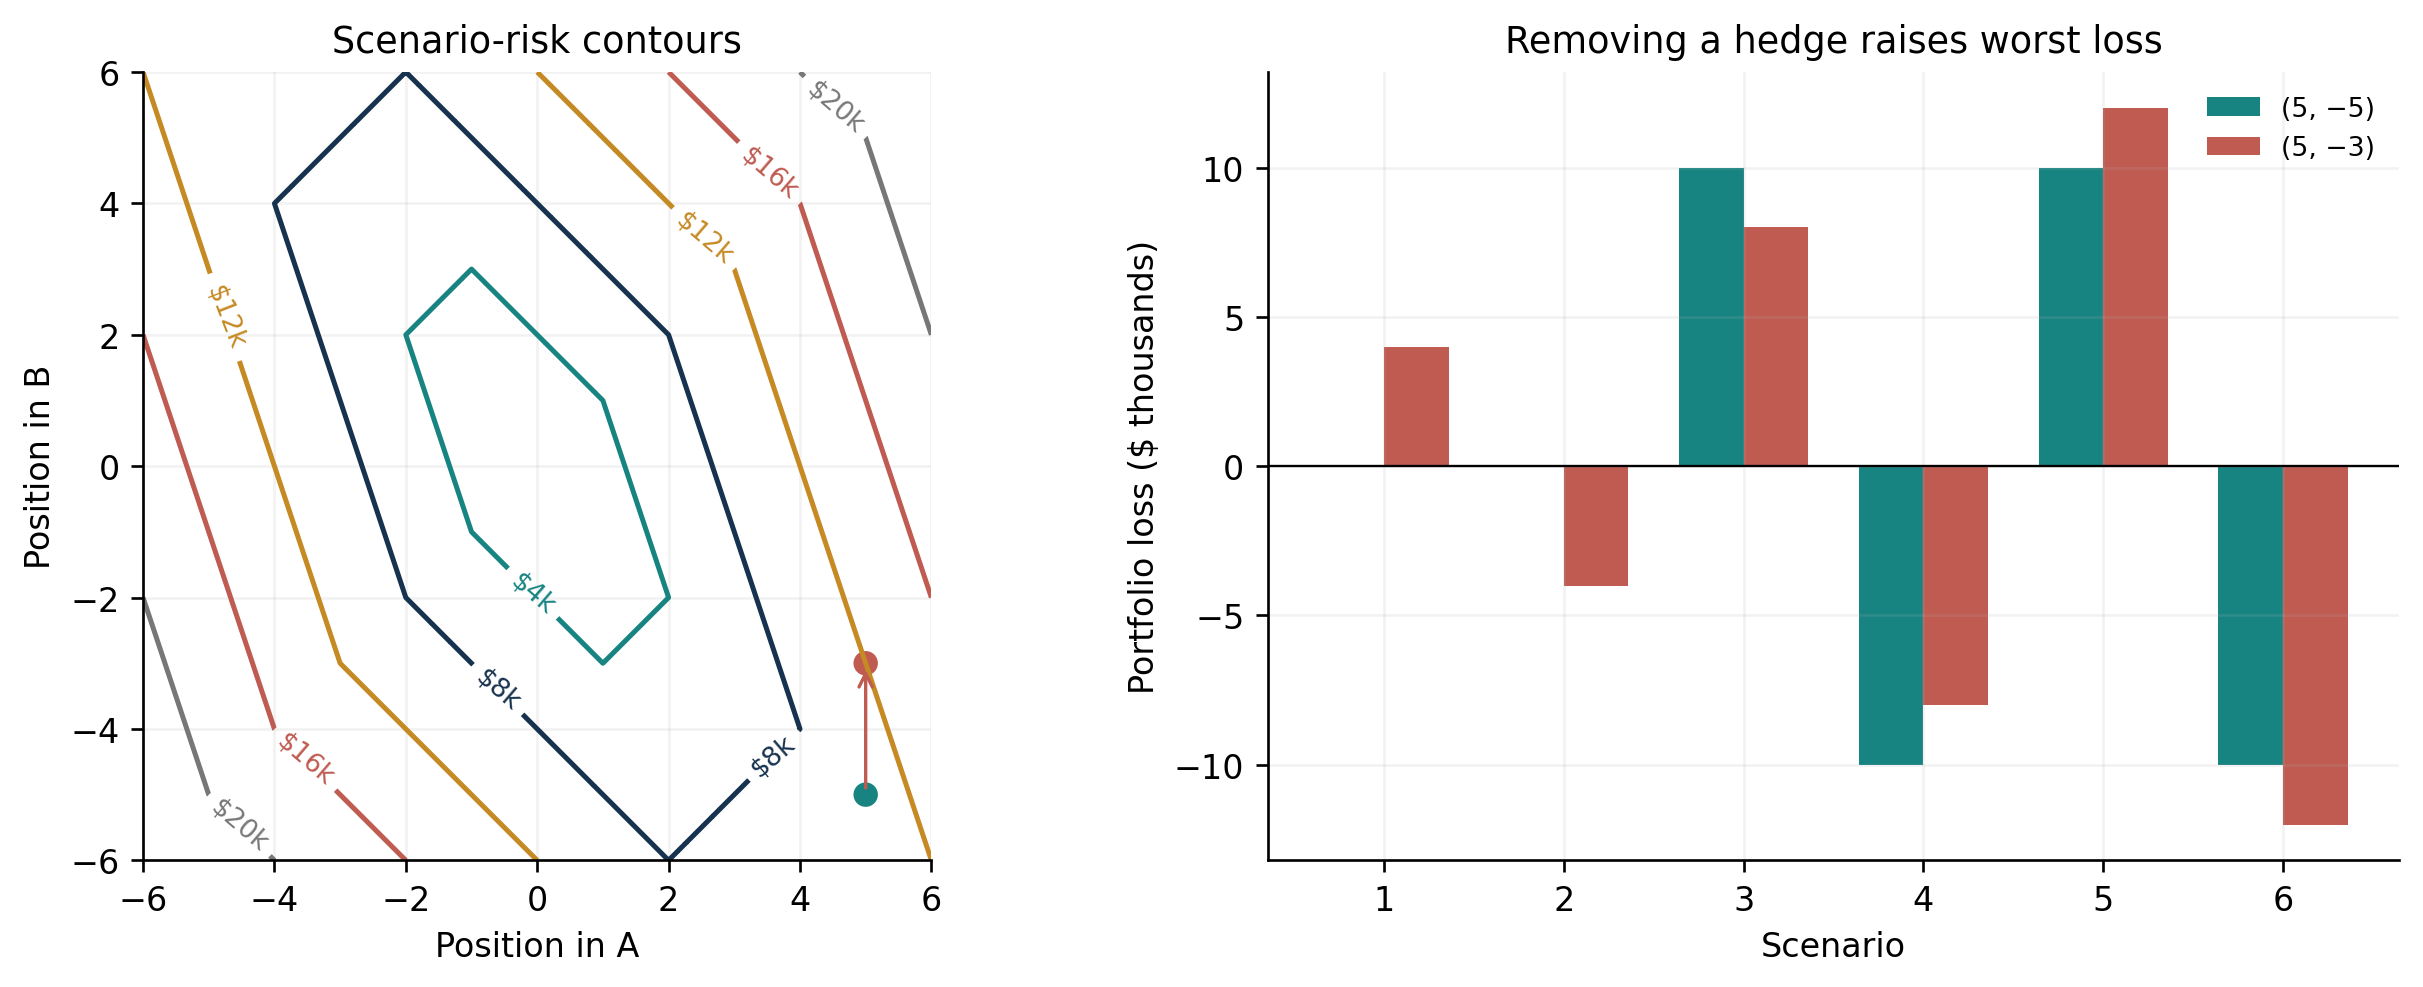
\includegraphics[width=\textwidth]{figures/07_margin.png}
\caption{Risk contours and scenario losses for the declared model. Moving from $(5,-5)$ to $(5,-3)$ crosses toward a larger worst-loss contour. Convexity in portfolio space is compatible with increased risk after removing one hedge leg.}
\label{fig:margin}
\end{figure}

\subsection{Historical quantiles and expected shortfall}

A historical value-at-risk calculation is a quantile, not generally a maximum. For scenario losses $L_s(z)=g_s^\top z$ with probabilities $\pi_s$, define
\begin{equation}
 \VaR_\alpha(z)=\inf\{a:\sum_{s:L_s(z)\le a}\pi_s\ge\alpha\}.
\end{equation}
A convex alternative, using the standard variational representation of \citet{Rockafellar2000}, is
\begin{equation}
 \ES_\alpha(z)=\min_{a\in\R}
 \left[a+\frac{1}{1-\alpha}\sum_s\pi_s\pos{L_s(z)-a}\right].
\label{eq:es}
\end{equation}
The representation handles discrete probability mass at the quantile by taking the required fraction of that mass. It should not be replaced with an unqualified conditional average over losses strictly above the quantile. For equal probabilities and a tail containing an integer number of observations, it is the average of that many largest losses. In Table~\ref{tab:risk}, at $(5,-3)$ and $\alpha=2/3$, the six-scenario VaR is \$4,000 while expected shortfall is $(8000+12000)/2=\$10,000$. The worst loss is \$12,000.

Convexity cannot be inferred from the word ``VaR.'' To see this directly, let two disjoint events each have probability 0.04. One position loses 100 only on the first event and a second loses 100 only on the second. Each has 95\% VaR zero, but their combined loss has 95\% VaR 100. The midpoint portfolio has VaR 50, violating convexity relative to the two individual positions. Hence Proposition~\ref{prop:risk} is a property of its declared risk functional, not a theorem about any production historical-quantile margin system.

\subsection{Which sensitivity is being measured?}

At least three sensitivities should be separated: a portfolio changes with risk parameters fixed; market conditions change and the risk parameters are recomputed; or available collateral changes while the required margin remains fixed. A large variation payment can coincide with any of these. The first sensitivity is described by $R$ and $M$ above. The second needs a model for $\theta_t$. The third is a resource-feasibility question, considered next.
\FloatBarrier
